\chapter{Cycle Gan e GradCam}
In questo capitolo illustreremo l'architettura del nostro progetto e andremo ad analizzare il codice. Partiremo con la definizione del problema della traduzione da immagine a immagine e vedremo com'è composta la rete che abbiamo utilizzato.

\section{Image to Image Translation}
(Ho pensato di strutturarla così: breve introduzione sul problema, spiegazione sul perchè pix2pix non sia la soluzione che usiamo, introduzione a cyclegan)\\
Vi siete mai chiesti come sarebbe bello poter ottenere una foto a colori da una foto in bianco e nero? Oppure avere la possibilità di passare da una foto ritraente un paesaggio estivo a un paesaggio autunnale?
\\Questi sono solamente alcuni degli esempi di applicazioni della traduzione da immagine a immagine. La traduzione da immagine ad immagine è molto simile a ciò che accade nella traduzione da lingua a lingua: partendo da un'immagine appartenente ad un dominio iniziale, come la foto di un paesaggio estivo, vogliamo ottenere un'immagine appartenente ad un altro dominio, ad esempio passando da paesaggio estivo a paesaggio autunnale.
\\Un esempio di traduzione da immagine a immagine è il già trattato Pix2Pix che, grazie ad una GAN condizionata addestrata con un training set paired, di cui un esempio in figura \ref{fig:Paired and Unpaired training set}, produce un output condizionato dall'immagine di input.
\\Tuttavia, l'approccio Pix2Pix fin qui descritto non è del tutto efficiente in quanto il training set della rete comporta un notevole sforzo nella sua creazione. Infatti, tornando all'esempio dei paesaggi, occorrebbe avere un enorme quantitativo di foto ritraenti lo stesso identico paesaggio in due differenti momenti dell'anno. In aggiunta, per alcune applicazioni sarebbe del tutto impossibile ottenere un training set di questo tipo: basti pensare alla traduzione da opere d'arte a foto, o all'applicazione di uno stile a immagini reali, come vedremo più avanti nel nostro caso quando vorremo trasformare cavalli in zebre e viceversa.

\begin{figure}[H]
  \begin{center}
    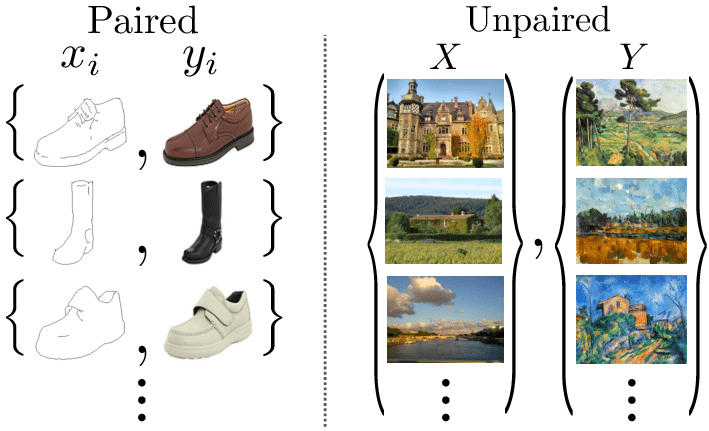
\includegraphics[width=0.8\columnwidth]{images/Paired-training-data-left-consists-of-training-examples-x-i-y-i-N-i1-where-the.png}
  \end{center}
  \caption{Vediamo un esempio di set paired, dove le immagini sono accoppiate tra input-outpu e set unpaired dove non vi è questa corrispondenza.}
  \label{fig:Paired and Unpaired training set}
\end{figure}
Proprio per questo motivo si è pensato di adottare una nuova soluzione attraverso l'addestramento con un training set \emph{unpaired}, dove non vi è una corrispondenza di input-output accoppiati, come vediamo sempre in figura \ref{fig:Paired and Unpaired training set}. In questo caso l'obiettivo è quello di addestrare una rete in grado di mappare le immagini appartenenti al dominio di partenza nel dominio di arrivo, in modo tale che le immagini generate siano verosimilmente appartenenti al dominio di arrivo.
\\Tuttavia non siamo ancora arrivati ad un risultato ottimale che soddisfi le nostre esigenze per la traduzione di un'immagine: in questo modo, infatti, non stiamo garantendo la traduzione esatta da immagine di input a immagine di output, ne stiamo solo condizionando la creazione. Inoltre potrebbe subentrare il problema del collasso della rete, dove tutte le immagini di input si mappano nella stessa immagine di output \cite{Zhu_2017_ICCV}.
Occorre quindi trovare un modo per migliorare l'idea fin qui realizzata, e proprio per questo motivo introduciamo una nuova architettura: la Cycle GAN.

\section{Cycle GAN}
(Ho pensato di strutturarla così: introduzione, spiegazione matematica del funzionamento della consistenza del ciclo, implementazione per la classe networks.py e cycle-gan-model.py (solo le funzioni importanti), addestramento)\\
Per spiegare questa architettura possiamo fare un paragone con la linguistica. Quando vogliamo tradurre una frase dall'italiano all'inglese vogliamo che applicando il procedimento di traduzione inversa da inglese a italiano, la frase torni ad essere quella di partenza. Vogliamo cioè che vi sia della consistenza tra i risultati. Questo concetto è ciò proprio che vogliamo applicare al nostro problema della traduzione da immagine a immagine. In poche parole vogliamo ottenere un'immagine di output, la quale applicando a ritroso la traduzione ci restituisca come risultato l'immagine di input. 
\\Matematicamente non vogliamo far altro che trovare due funzioni biettive $G:X\rightarrow{}Y$ e $F:Y\rightarrow{}X$, tali per cui $F$ sia l'inversa di $G$, ovvero:
$$\begin{cases}
  F(G(x))=x\\
  G(F(y))=y  
\end{cases}
$$
Da un punto di vista architetturale questo problema può essere risolto attraverso due reti GAN, la prima responsabile della traduzione da $X$ a $Y$, la seconda resposabile della traduzione inversa da $Y$ a $X$ \cite{Zhu_2017_ICCV}. In questo modo il generatore della prima rete prenderà in input le immagini dal primo dominio e produrrà in output le immagini per il secondo dominio, successivamente il compito passerà al generatore della seconda rete che prenderà come input le immagini generate dal primo generatore e produrrà come output un'immagine del primo dominio il più fedele possibile, poi vedremo come, all'immagine di partenza. I rispettivi discriminatori saranno impiegati nel determinare quanto le immagini generate siano plausibili. 
\\Per quanto riguarda l'addestramento, esso è conforme a quanto già descritto per le reti GAN, con l'aggiunta di una loss che indica la consistenza del ciclo. Per spiegare come viene calcolata questa loss aggiuntiva definiamo due concetti: \emph{forward cycle consistency} e \emph{backward cycle consistency}. Il forward cycle consistency (consistenza del ciclo in avanti) non è altro che la sopra definita $F(G(x))=x$, mentre il backward cycle consistency (consistenza del ciclo all'indietro) è la sopra definita $G(F(Y))=y$, come si può intuire visivamente dalla figura \ref{fig:Cycle Consistency}. Attraverso questi due concetti possiamo quindi valutare di quanto si discosta l'immagine rigenerata, grazie al forward cycle consistency, con l'immagine iniziale. Infatti, calcolando la differenza (che matematicamente rappresentiamo con la norma, o la norma al quadrato) tra le due immagini si ottiene l'errore che la rete commette durante la traduzione dell'immagine. Possiamo applicare il medesimo ragionamento per quanto riguarda il backward cycle consistency per ottenere la loss di consistenza del ciclo:
$$L\textsubscript{cyc}(G,F) = ||G(F(x))-x|| + ||F(G(Y))-y||$$

\begin{figure}[H]
  \begin{center}
    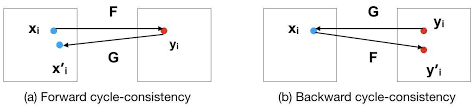
\includegraphics[width=0.8\columnwidth]{images/cycle consistency.png}
  \end{center}
  \caption{Vediamo una rappresentazione grafica della consistenza del ciclo.}
  \label{fig:Cycle Consistency}
\end{figure}
In questo modo abbiamo quindi definito una rete costituita da due GAN cicliche, da cui il nome. La loss totale della rete dipenderà quindi dalle loss delle due GAN, più la loss aggiuntiva che indica la consistenza del ciclo.
$$L\textsubscript{cycgan}(G,F,D\textsubscript{x},D\textsubscript{y})=
L\textsubscript{gan}(G,D\textsubscript{y},X,Y) +
L\textsubscript{gan}(F,D\textsubscript{x},Y,X) + 
L\textsubscript{cyc}(G,F)
$$
Come ampiamente spiegato la Cycle GAN può essere definita attraverso due funzioni biettive, una l'inversa dell'altra. Un problema di traduzione da immagine a immagine risolto attraverso l'implementazione di una rete di questo tipo porterà quindi ad una doppia soluzione: la traduzione, che possiamo definire \emph{primaria}, da dominio $A$ a dominio $B$ ed una traduzione \emph{secondaria} da dominio $B$ a dominio $A$.
Vedremo infatti nei capitoli futuri come il nostro progetto si concentri sulla traduzione di immagini da cavalli a zebre, ma noteremo come, seppur con risultati inferiori, la rete sia in grado di tradurre anche da zebre a cavalli, come vediamo tra gli esempi di figura \ref{fig:Cycle GAN Example}.

\begin{figure}[H]
  \begin{center}
    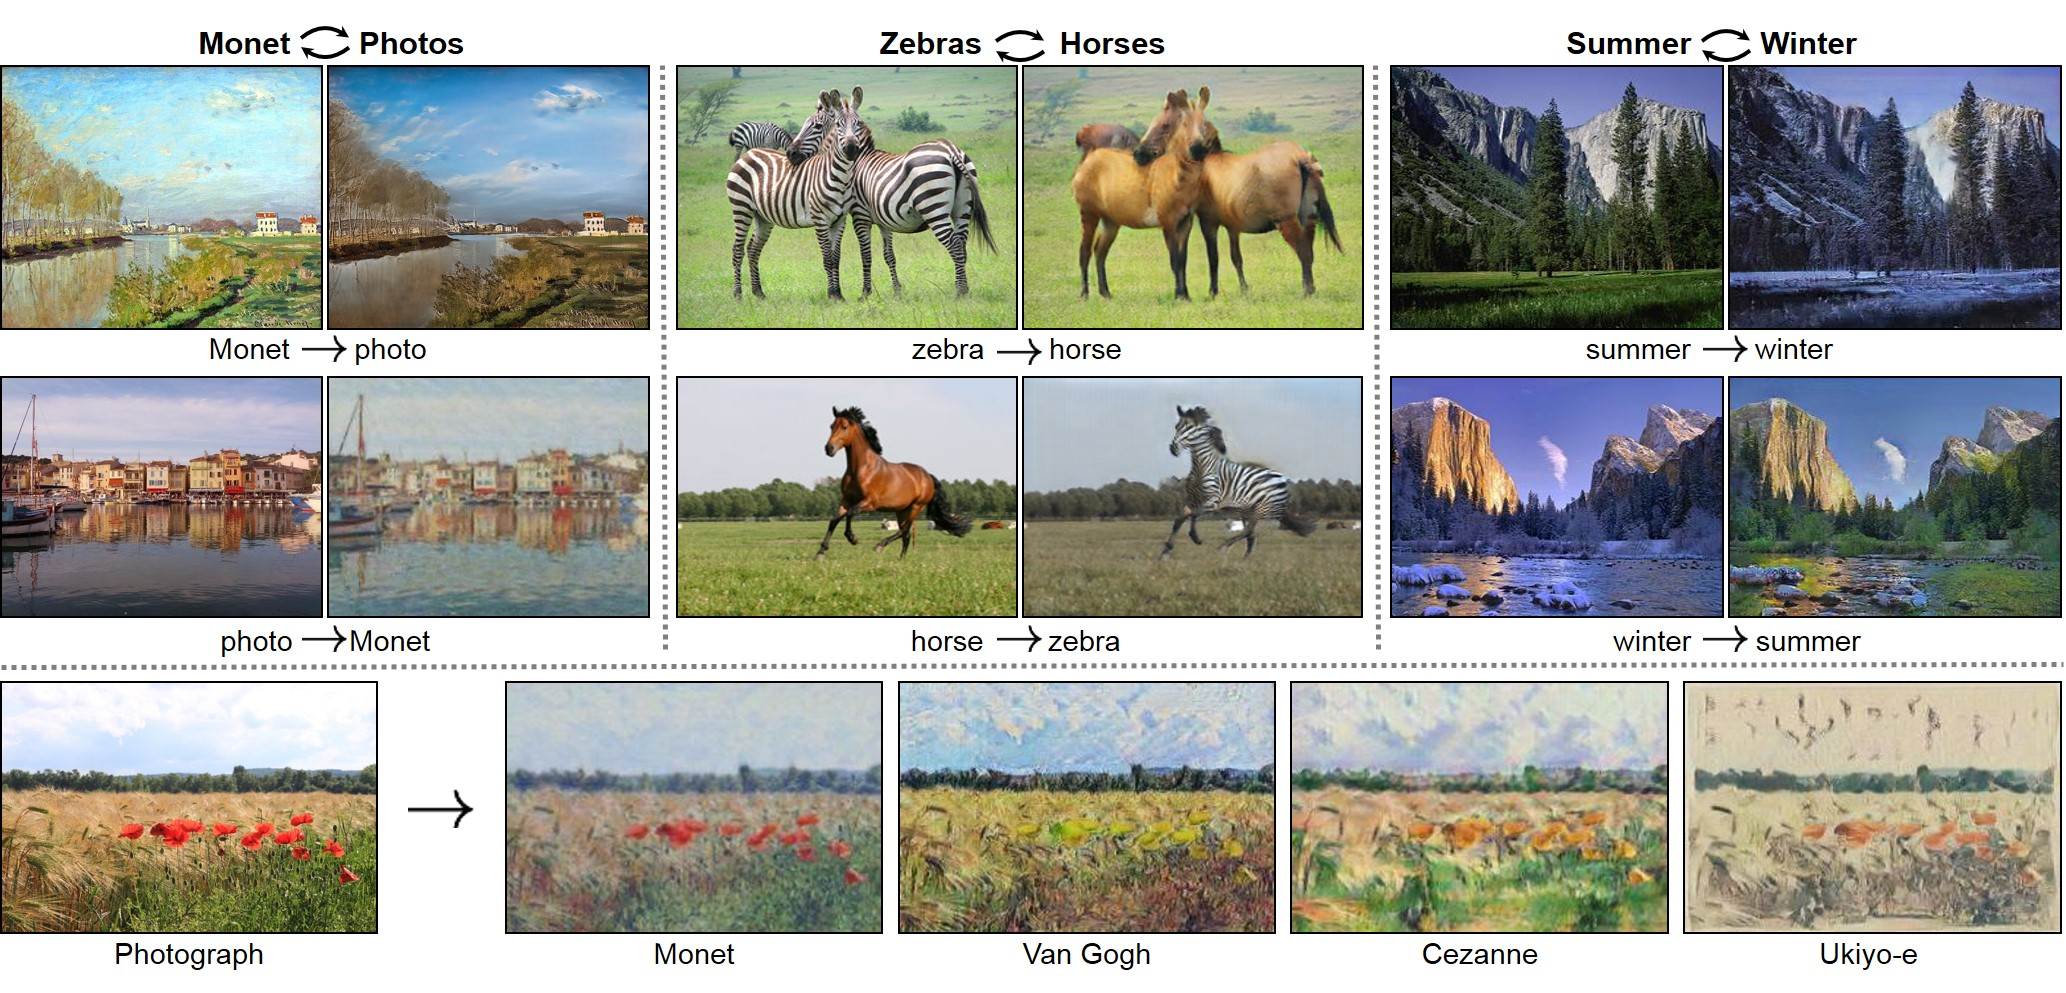
\includegraphics[width=1\columnwidth]{images/cycle gan example.jpg}
  \end{center}
  \caption{Vediamo vari esempi di una image to image translation attraverso l'uso di Cycle GAN.}
  \label{fig:Cycle GAN Example}
\end{figure}

\section{Codice ed Implementazione}
Dopo aver trattato la teoria sulla quale si basano le Cycle GAN vediamo in questa sezione com'è possibile implementarle a livello di codice. L'implementazione iniziale da cui partiremo è quella proposta dal  \href{https://github.com/junyanz/pytorch-CycleGAN-and-pix2pix}{Paper} \cite{Zhu_2017_ICCV}.
\\Il codice è scritto in Python e utilizza il Framework Pytorch per costruire la rete e addestrarla. Il codice dà la possibilità di specificare diversi parametri utili alla rete, in questa sezione ci limiteremo a definire quelli utilizzati nel nostro progetto.
\subsection{Networks}
La prima classe che andiamo a definire è la classe \href{https://github.com/junyanz/pytorch-CycleGAN-and-pix2pix/blob/master/models/networks.py}{networks}, all'interno della quale vengono definite le architetture utilizzate per implementare la CycleGAN.
Come prima cosa andremo a definire le reti Generatrici, che nel nostro progetto saranno composte attraverso un'architettura ResNet avente nove blocchi residui. Notiamo come durante l'inizializzazione del Generatore sia possibile andare a specificare alcuni parametri, per cambiare il comportamento della rete. Tra questi troviamo la tipologia dell'architettura utilizzata, la quale, nel nostro caso, sarà, come detto, una ResNet.

\begin{minted}[bgcolor=lightGray]{python}
def define_G(input_nc, output_nc, ngf, netG, norm='batch',
            use_dropout=False, init_type='normal',             
            init_gain=0.02, gpu_ids=[]):
                
    norm_layer = get_norm_layer(norm_type=norm)

    if netG == 'resnet_9blocks':
        net = ResnetGenerator(input_nc, output_nc, ngf,
                            norm_layer=norm_layer,
                            use_dropout=use_dropout,
                            n_blocks=9)
\end{minted}
Con codice analogo vengono successivamente definite le reti Discriminatrici. Anche in questo caso sarebbe possibile specificare ulteriori parametri per cambiare il tipo di rete utilizzato. Si distinguono tre tipologie di Discriminatore: \emph{basic}, \emph{n-layer} e \emph{pixel}. Nella nostra rete utilizzeremo il discriminatore Basic, il quale suddivide l'immagine in parti composte da 70x70 pixel e per ognuna di queste viene effettuata una classificazione tra reale e fake.
\\Successivamente viene definita la Loss della GAN, nel nostro progetto utilizzeremo una MSELoss.
\begin{minted}[bgcolor=lightGray]{Python}
 def __init__(self, gan_mode, target_real_label=1.0,
                 target_fake_label=0.0):
    if gan_mode == 'lsgan':
        self.loss = nn.MSELoss()
\end{minted}
Proseguendo all'interno del codice vengono definiti i blocchi residui della nostra ResNet. Come detto in precedenza la nostra rete sarà composta da nove blocchi residui. I blocchi residui vengono utilizzati nel Deep Learning al fine di poter ottenere una maggiore profondità della rete. Infatti, se anzichè utilizzare una ResNet utilizzassimo un'altra architettura, sarebbe errato parlare di precisione della rete proporzionale alla sua profondità, in quanto subentrerebbe il problema del \emph{gradiente di fuga}, secondo il quale il gradiente si annullerà a causa dei troppi livelli. Per questo motivo vengono introdotte le ResNet, le quali attraverso \emph{salti} tra i layer che compongono i blocchi residui, riescono ad evitare questo problema \cite{targ2016resnet}.
\\Ogni blocco residuo è composto da i seguenti layer:
\begin{minted}[bgcolor=lightGray]{Python}
ResnetBlock(
    (conv_block): Sequential(
      (0): ReflectionPad2d
      (1): Conv2d
      (2): InstanceNorm2d
      (3): ReLU
      (4): ReflectionPad2d
      (5): Conv2d
      (6): InstanceNorm2d
    )
\end{minted}
\subsection{Cycle GAN Model}
Dopo aver descritto come viene definita l'architettura della rete, possiamo descrivere come la Cycle GAN è implementata. 
\\Come prima cosa occorre ovviamente costruire i due generatori e i due discriminatori, richiamando i sopra citati metodi della classe networks:
\begin{minted} [bgcolor=lightGray] {Python}
self.netG_A = networks.define_G(opt.input_nc, opt.output_nc,
                        opt.ngf, opt.netG, opt.norm,
                        not opt.no_dropout, opt.init_type,
                        opt.init_gain, self.gpu_ids)
self.netG_B = networks.define_G(opt.output_nc, opt.input_nc,
                        opt.ngf, opt.netG, opt.norm,
                        not opt.no_dropout, opt.init_type,
                        opt.init_gain, self.gpu_ids)
self.netD_A = networks.define_D(opt.output_nc, opt.ndf,
                        opt.netD,opt.n_layers_D, opt.norm,
                        opt.init_type, opt.init_gain,
                        self.gpu_ids)
self.netD_B = networks.define_D(opt.input_nc, opt.ndf,
                        opt.netD,opt.n_layers_D, opt.norm,
                        opt.init_type,opt.init_gain,
                        self.gpu_ids)
\end{minted}
Successivamente definiamo il comportamento dei Generatori che avranno il compito di generare le immagini fake attraverso le quali andremo a calcolare la Loss:
\begin{minted}[bgcolor=lightGray]{Python}
def forward(self):
    self.fake_B = self.netG_A(self.real_A)  # G_A(A)
    self.rec_A = self.netG_B(self.fake_B)   # G_B(G_A(A))
    self.fake_A = self.netG_B(self.real_B)  # G_B(B)
    self.rec_B = self.netG_A(self.fake_A)   # G_A(G_B(B))
\end{minted}
Come vediamo le istruzioni rappresentano il funzionamento descritto per le Cycle GAN: partendo da un'immagine del dominio $A$, generiamo con il primo generatore un'immagine fake per il dominio $B$, successivamente attraverso il secondo generatore ricostruiamo l'immagine iniziale partendo dall'immagine fake del dominio $B$. Questo procedimento è ripetuto in maniera analoga anche per la generazione da dominio $B$ a dominio $A$.
\\Seguentemente definiamo la funzione Backward per i due discriminatori, alla quale passiamo come argomenti le immagini reali e le immagini fake, su cui i discriminatori dovranno effettuare la previsione, al fine di calcolare la Loss dei discriminatori.
\begin{minted}[bgcolor=lightGray]{Python}
def backward_D_basic(self, netD, real, fake):
    pred_real = netD(real)
    loss_D_real = self.criterionGAN(pred_real, True)
    # Fake
    pred_fake = netD(fake.detach())
    loss_D_fake = self.criterionGAN(pred_fake, False)
    # Combined loss and calculate gradients
    loss_D = (loss_D_real + loss_D_fake) * 0.5
    loss_D.backward()
\end{minted}
Infine definiamo il metodo di Backward per quanto riguarda i generatori: è qui che calcoleremo la Loss di consistenza del ciclo. 
\begin{minted}{Python}
# Forward cycle loss || G_B(G_A(A)) - A||
self.loss_cycle_A = self.criterionCycle(self.rec_A, self.real_A)
# Backward cycle loss || G_A(G_B(B)) - B||
self.loss_cycle_B = self.criterionCycle(self.rec_B, self.real_B)
\end{minted}
Oltre alla Loss di consistenza del ciclo sono ovviamente presenti le classiche Loss per le reti GAN e una Loss di identità ottenuta passando ad un generatore un'immagine del dominio di arrivo, teoricamente il generatore in questione dovrebbe produrre come output l'immagine stessa in quanto già appartenente al dominio d'arrivo.

\section{Addestramento}
Abbiamo quindi definito tutti i punti più importanti delle classi che definiscono la nostra rete, ora possiamo concentrarci sull'addestramento. Per prima cosa occorre definire un dataset sul quale andare a lavorare. Il progetto dal quale siamo partiti mette a disposizione svariati dataset su cui addestrare la rete, tra questi il dataset \emph{horse2zebra}. Il dataset in questione offre la possibilità di tradurre immagini di cavalli in zebre, quindi applicando le strisce bianche e nere al manto del cavallo, e da zebre a cavalli, quindi applicando il procedimento inverso rimuovendo le strisce bianche e nere e dando un colore omogeneo al manto.
\\Per l'addestramento della rete si è scelto di utilizzare Google Colab, un ambiente gratuito offerto dalla Google che mette a disposizione le proprie schede grafiche per addestrare reti di questo tipo. 
\\L'addestramento si basa su epoche e per la nostra rete il numero di epoche fissato è pari a 200.
\\Per quanto riguarda i tempi di addestramento essi ovviamente variano a seconda della rete che si vuole addestrare. Nel nostro caso i tempi impiegati dalla Cycle GAN fin qui descritta erano dell'ordine dei minuti per epoca, indicativamente dieci. Per le modifiche successive che apporteremo alla rete vedremo come il tempo necessario all'addestramento aumenterà, fino ad arrivare a oltre quaranta minuti per epoca per la Cycle GAN addestrata grazie all'utilizzo di GradCam su quattro blocchi residui, che descriveremo nei capitoli successivi.
\\(parlo qui delle modifiche che ho fatto io al codice, quindi aggiungendo una sezione contenente la spiegazione di GradCam.py e di come collabori con cycle-gan-model.py, oppure lo faccio nel prossimo capitolo?)

\section{GradCam}
Nel capitolo precedente abbiamo trattato l'algoritmo GradCam definendolo come un algoritmo in grado di associare una risposta visiva al comportamento della rete, indicandoci attraverso una mappa di calore dove la rete pone la propria attenzione durante la generazione delle immagini. L'idea è quindi quella di sfruttare GradCam al fine di indirizzare l'attenzione della rete durante la generazione delle immagini. Idealmente, infatti, le mappe di attenzione durante la ricostruzione dell'immagine iniziale, quindi dal dominio $B$ al dominio $A$, dovrebbero essere uguali a quelle della trasformazione da $A$ a $B$. Infatti, tornando all'esempio del dataset cavalli e zebre, ci aspettiamo che se la mappa di attenzione generata dalla rete durante la trasformazione da cavallo a zebra si focalizza sulla sagoma del cavallo per inserirne le strisce bianche e nere, anche l'attenzione generata dalla ricostruzione da zebra fake a cavallo si focalizzi negli stessi punti della precedente, in modo tale da rimuovere le strisce aggiunte e riportare il manto del cavallo allo stato iniziale. Il ragionamento è molto simile alla già illustrata consistenza del ciclo per le CycleGAN: deve esserci consistenza tra le mappe di attenzione. Lo scopo del nostro progetto è dunque quello di introdurre una nuova loss che indichi questa uguaglianza. 

\subsection{Implementazione}
Vediamo ora come applicare il ragionamento fin qui spiegato. Come prima cosa occorre definire i parametri su cui lavora GradCam. Come già accennato nei capitoli precedenti, GradCam lavorà sui layer di una rete, quindi occorrerà scegliere tra i layer che compongono la nostra rete quelli sui quali andare a generare le mappe di attenzione. Oltre a questo, occorre andare a definire qual è l'output di classificazione su cui effettuare la backpropagation. Nel nostro caso non abbiamo un vero e proprio output di classificazione, ma possiamo sfruttare l'output del Discriminatore come tale. Infatti il comportamento del Discriminatore è molto simile ad un classificatore: possiamo vedere la determinazione tra immagine vera o immagine fake come una vera e propria classificazione. 
\\Abbiamo quindi definito tutti i parametri fondamentali per implementare GradCam in una CycleGAN, possiamo concentrarci ora sull'analisi delle istruzioni fondamentali.
Prima di procedere con l'analisi del codice, però, dobbiamo definire su quali layer ricavare le mappe di attenzione da utilizzare per il calcolo della Loss sopra citata. La rete generatrice, infatti, è composta da 23 blocchi sui quali è possibile andare a generare le mappe di attenzione. Idealmente, si potrebbero utilizzare tutti e 23 i layer, magari associando un peso diverso per ognuni di essi, ma non è una strada ottimale, in quanto non tutti i layer sono utili al nostro scopo. La scelta dei layer su cui calcolare la Loss ricade quindi sui nove blocchi residui della rete, in quano come vediamo in figura \ref{fig:GradCam Horse},  sono i layer che offrono i risultati migliori. Come vedremo successivamente, i risultati migliori sono quelli ottenuti utilizzando solo l'ultimo blocco residuo per calcolare la Loss di consistenza dell'attenzione. 

\begin{figure}[H]
  \begin{center}
    \includegraphics[width=0.8\columnwidth]{images/gradCam horse.png}
  \end{center}
  \caption{Vediamo le varie mappe di attenzione generate applicando GradCam su tutti i blocchi possibili della rete.}
  \label{fig:GradCam Horse}
\end{figure}

\subsection{Codice}
Dopo aver definito tutti i parametri sui quali lavorare possiamo soffermarci sul codice necessario a realizzare quanto spiegato fin'ora. 
Definiamo in primo luogo la classe FeatureExtractor, la quale ha il compito di salvare il gradiente dei layer scelti per generare le mappe di attenzione. 
\begin{minted}[bgcolor=lightGray] {Python}
def __init__(self, model, target_layers):
    self.model = model
    self.target_layers = target_layers
    self.gradients = []
def __call__(self, x):
    outputs = []
    self.gradients = []
    for name, module in self.model._modules.items():
        x = module(x)
        if name in self.target_layers:
            x.register_hook(self.save_gradient)
            outputs += [x]
    return outputs, x
\end{minted}
Come vediamo scorriamo tutti i layer della rete e li applichiamo all'immagine $x$. Successivamente verifichiamo se il layer in questione è tra quelli sui quali vogliamo generare le mappe di attenzione: in caso affermativo salviamo il gradiente e ne salviamo l'output in uscita dal Generatore, precedentemente calcolato, in una lista.
\\Successivamente definiamo la classe ModelOutputs, che ha il compito di sfruttare l'output del Discriminatore per generare le mappe di attenzione.

\begin{minted}[bgcolor=lightGray]{Python}
class ModelOutputs():
    def __init__(self, model, discriminator, feature_module,
                target_layers):
        self.model = model
        self.feature_module = feature_module
        self.discriminator = discriminator
        self.feature_extractor =
        FeatureExtractor(self.feature_module,
                        target_layers)

    def get_gradients(self):
        return self.feature_extractor.gradients

    def __call__(self, x):
        target_activations = []
        for name, module in self.model._modules.items():
            if module.model == self.feature_module:
                target_act, x = self.feature_extractor(x)
            elif "avgpool" in name.lower():
                x = module(x)
                x = x.view(x.size(0),-1)
            else:
                x = module(x)
                x = self.discriminator(x)
        return target_act, x

\end{minted}
Vediamo come si scorrano tutti i layer del Generatore e per ognuno di essi si verifichi se è tra quelli su cui vogliamo generare l'attenzione: in caso affermativo, viene salvato il gradiente, grazie alla classe FeatureExtractor sopra citata. Infine, per ogni layer ne viene calcolato l'output, generando quindi l'immagine fake. L'immagine generata viene di conseguenza passata al discriminatore, al fine di determinare l'output di classificazione necessario a GradCam per generare le mappe di attenzione.
Infine, definiamo la classe GradCam avente il compito di generare, grazie all'utilizzo delle classi precedenti, le mappe di attenzione.
Dopo aver richiamato il metodo dell'estrazione delle features, determiniamo un tensore \emph{one\_hot} contente la media dei valori di classificazione determinati dal Discriminatore su cui andiamo a fare la backpropagation. Successivamente, andiamo a definire il tensore \emph{grads\_val}, attraverso il quale andiamo a recuperare i gradienti precedentemente salvati. Infine, tramite questi gradienti, viene definita la mappa di attenzione \emph{cam} cercata.
\begin{minted}[bgcolor=lightGray]{Python}
    features, output = self.extractor(input)
    one_hot = torch.mean(output)
    
    one_hot.backward(retain_graph=True)

    grads_val = self.extractor.get_gradients()[-1].cpu().data

    target = features[-1]
    target = target.cpu().data[0, :]

    weights = torch.mean(grads_val, axis=(2, 3))[0, :]
    cam = torch.zeros(target.shape[1:], dtype=torch.float32)

    for i, w in enumerate(weights):
        cam += w * target[i, :, :]

    cam = F.relu(cam)
    cam = cam - torch.min(cam)
    cam = cam / torch.max(cam)
    return cam
\end{minted}

\subsection{CycleGAN e GradCam}
Ora, come ultimo passaggio non ci resta che combinare insieme le due architetture fin qui definite, al fine di poter calcolare la Loss di consistenza dell'attenzione. Per fare questo quindi generiamo le mappe di attenzione all'interno della classe cycleGan model sia sulla traduzione da $A$ a $B$ che nella ricostruzione da $B$ a $A$. 
\begin{minted}[bgcolor=lightGray]{Python}
def __init__(self, opt):
    self.gradcamG_A = GradCam(model=self.netG_A,
                    discriminator=self.netD_A,
                    feature_module=self.netG_A.module.model,
                    use_cuda=True)
    self.gradcamG_B = GradCam(model=self.netG_B,
                    discriminator=self.netD_B,
                    feature_module=self.netG_B.module.model,
                    use_cuda=True)
    
def forward(self):
    self.fake_B = self.netG_A(self.real_A)
    horse = self.real_A.requires_grad_(True)   
    self.cam_fake_B = self.gradcamG_A(horse,self.first_layer,
                                    None)
    self.cam_fake_B = self.cam_fake_B.unsqueeze(0)
    for name in (self.layers):
        self.cam_fake_B = torch.cat((self.gradcamG_A(horse,
                                    name,None).unsqueeze(0),
                                    self.cam_fake_B),dim=0)
    
\end{minted}
Come vediamo dal codice, generiamo le mappe di attenzione sull'immagine reale per ogni layer tra quelli da noi indicati. Questa operazione viene ripetuta, ovviamente con i rispettivi generatori e discriminatori, anche per l'immagine ricostruita e per la traduzione inversa da zebre a cavalli.
\\Concludiamo ora la parte relativa al codice andando ad implementare la Loss di consistenza dell'attenzione. Per calcolarla utilizziamo una \emph{MSELoss}, ovvero la norma al quadrato tra le due attenzioni generate.
\begin{minted}[bgcolor=lightGray]{Python}
def backward_G(self):
    self.att_lossA2B = self.MSE_LOSS(self.cam_fake_B.detach(),
                                    self.cam_rec_A)
    self.att_lossB2A = self.MSE_LOSS(self.cam_fake_A.detach(),
                                    self.cam_rec_B)
\end{minted}
Analizzeremo successivamente il perchè vi sia un \emph{detach} sulle mappe di attenzione delle immagine fake.